\begin{abstract}
	L'obiettivo dell'esperienza è la misura della costante di assorbimento del mylar.
	Tale misura è stata effettuata misurando le tensioni generate in un fotodiodo in funzione della luce trasmessa attraverso vari spessori di mylar.
	
	Essendo tali misurazioni fortemente perturbate da rumori ambientali e strumentali
	si è proceduto alla realizzazione di un amplificatore sensibile alla frequenza con la tecnica del lock-in
	in maniera da aumentare il rapporto segnale/rumore.
	
	La costante di assorbimento del mylar è poi stata ottenuta attraverso un fit della 
	legge di Lambert per l'assorbimento di una radiazione da parte di un mezzo uniforme.
\end{abstract}

\section{Strumentazione}
La strumentazione usata è quella presente sul banco di lavoro, più:
\begin{itemize}
		\item i seguenti circuiti integrati:
		\begin{itemize}
			\item TL082: JFET input dual op-amp;
			\item quattro TL081: JFET input op-amp;
			\item SN7400: quad NAND gates;
			\item DG441: quad CMOS analog switch;
			\item 2N1711,BC182: NPN transistor;
		\end{itemize}
			\item un LED rosso;
			\item un fotodiodo;
			\item varie lastrine di mylar dello spessore di $150$\si{\micro \metre} l'una.
	\end{itemize}
	
\section{Metodo di misura}
L'apparato sperimentale è schematizzato in \figurename{ \ref{f:complessivo}}.
	Tale circuito svolge la funzione di un amplificatore sensibile alla frequenza con la tecnica del lock-in in maniera da aumentare il segnale.
	Per la verifica del funzionamento circuitale si è proceduto effettuando un montaggio a blocchi
	e verificandone separatamente il funzionamento.
	
	Per limitare le fonti di rumore si è proceduto a collegare tra loro le varie linee di terra della breadboard,
	si sono impegati condensatori tra le linee di alimentazione della breadboard, i collegamenti sono stati realizzati quanto più corti e appiattiti possibile.
	\begin{figure}[ht]
		\centering
		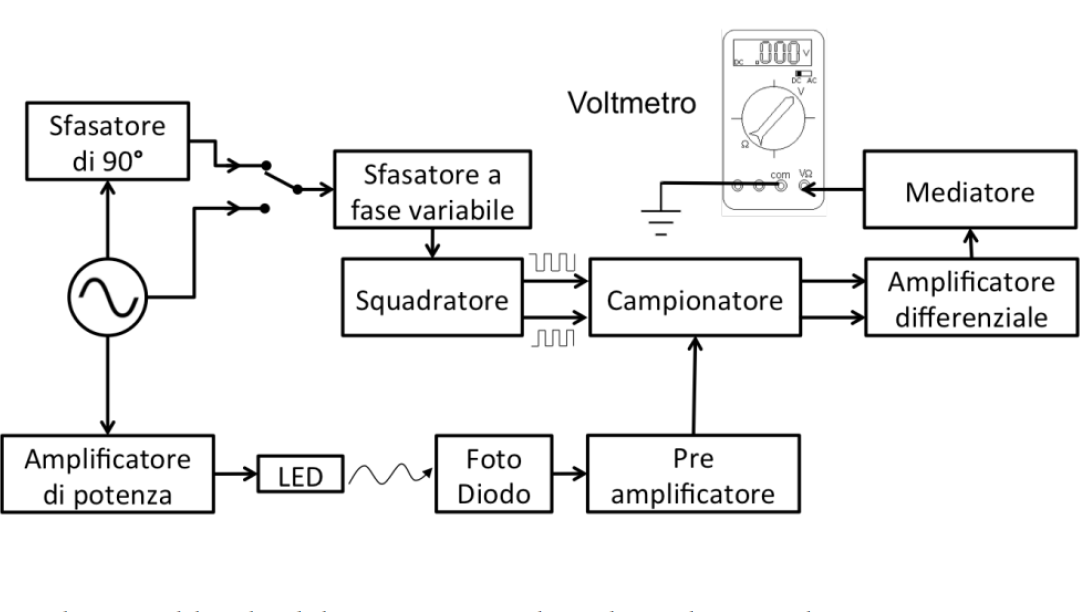
\includegraphics[scale=0.3]{./c1.png}
		\caption{scema del apparato strumentale usato.}
		\label{f:complessivo}
	\end{figure}
\paragraph{Setup}
	Sono state impiegate le tensioni di alimentazione 
	$V_{+}=$\SI{ 5.00 \pm 0.04}{\volt} e $V_{-}=$\SI{ -4.98 \pm 0.04}{\volt}
	e un segnale sinusoidale $S1$ di tensione $V_{pp}=$\SI{6.00\pm 0.04}{\volt} e $f=$\SI{1.0271 \pm 0.0001}{\kilo \hertz}.
